\chapter{Постановка задачи}

\section{Описание предметной области}

\subsection{Методики сравнения}
Визуальное сравнение изображений -- это процесс количественной оценки степени
визуального сходства между изображениями на основе извлекаемых из них
характеристик, с последующим ранжированием результатов. Можно выделить три
основных подхода к сравнению изображений: метрики структурного анализа,
хеширование изображений и использование машинного обучения.

\subsubsection{Метрики}
Метрика сходства -- это математическая абстракция для сравнения объектов,
присваивающая число, указывающее на степень родства между объектами указанной
пары \cite{ali2016survey}. Самый простой пример -- процент совпавших пикселей,
однако, существует множество более эффективных методов, различающихся по
сравниваемым признакам: цвет, текстура, форма и структура.

Метрики цвета количественно описывают распределение цветов и их статистические
характеристики в изображении. Чаще всего, речь о гистограммах. Гистограмма
изображения показывает частоту распределение пикселей различной интенсивности
показателя (цвет, освещенность и др.) \cite{ali2016survey}.

Метрики текстуры оценивают визуальные паттерны, структуру и неоднородности
поверхностей. Наиболее известны вейвлет"=преобразования. Вейвлет"=преобразование
одномерного сигнала состоит в его разложении по базису, сконструированному из
обладающей определенными свойствами солитоноподобной функции (вейвлета)
посредством масштабных изменений и переносов \cite{астафьева1996вейвлет}.

Метрики формы смотрят на геометрические и контурные особенности объектов.
Обычно, используются дескрипторы, такие как \textit{SIFT} (сравнение наборов
особых точек, найденных с помощью пирамиды гауссианов и ее разностей)
\cite{lowe2004distinctive}.

Наиболее популярны структурные метрики. Они позволяют оценить сходство
изображений по взаимосвязи между элементами. Каноничным примером алгоритма не
только структурного сравнения, но и визуального сравнения в целом считается,
имеющий десятки модификаций, \textit{SSIM} -- развитие методов \textit{RSNR} и
\textit{MSE}, с учетом специфики \textquote{восприятия ошибки}
\cite{wang2004image}.

\subsubsection{Хеширование}
Перцептивное хеширование -- отличается от метрики сходства наличием
промежуточного шага. Сравниваются не объекты, а их хеши. Операция сравнения
хешей проста и высокоэффективна, за счет чего можно значительно снизить
вычислительную нагрузку, если нужно сравнить эталон со множеством паттернов.
Вычисление всегда начинается с масштабирования изображения до маленького
размера, а затем проводится некоторое преобразование этой квадратной матрицы, в
зависимости от варианта алгоритма, за которым следует создание хеша из элементов
взятых в любом порядке. Для сравнения используют косинусное или Евклидово
расстояние или расстояние Хэмминга \cite{zauner2010implementation}.

Наиболее известны варианты основанные на дискретном косинусном преобразовании
(\textit{DCT}) для выделения низкочастотных компонентов (основной вариант,
Перцептивный хеш, \textit{pHash})\cite{zauner2010implementation}, на среднем
значении яркости (\textit{Average Hash}, \textit{aHash}), хеш радиального
отклонения (\textit{Radial Variance Hash}, \textit{vrHash}) и вейвлет"=функции
(\textit{Wavelet Hash}, \textit{wHash}) \cite{zauner2010implementation}.

\subsubsection{Машинное обучение}
Выделяется пять нейросетевых методов сравнения, которые позволяют извлекать и
сравнивать высокоуровневые визуальные признаки, что дает значительные
преимущества по сравнению с традиционными подходами. Они требуют несравнимо
больше аппаратных ресурсов чем метрики, однако гарантируют большую точность и
позволяют сравнивать смысловое содержание изображений: одинаковый ли объект (тип
объектов) на них изображен и на сколько они похожи.

Сети для извлечения дескрипторов обучаются извлекать компактные числовые
дескрипторы, описывающие визуальные характеристики изображений. Примером таких
сетей служит \textit{ResNet}\cite{simonyan2015deep}.

Сиамские нейронные сети состоят из двух или более идентичных подсетей, которые
обрабатывают несколько изображений параллельно; их обучают определять, являются
ли два изображения похожими или нет, на основе сравнения их внутренних
представлений \cite{koch2015siamese}.

Генеративные модели, например \textit{DCGAN}, могут сравнивать изображения на
основе их внутренних представлений \cite{radford2015unsupervised}.

Сети с контрастивным обучением используют методы контрастивного обучения для
различения похожих и непохожих изображений путем сравнения их внутренних
признаков, подобные \textit{SimCLR} \cite{DBLP:journals/corr/abs-2002-05709}.

Сети для семантической сегментации, такие как \textit{U-Net}, сравнивают
структуры и содержания на основе сегментированных областей
\cite{10.1007/978-3-319-24574-4_28}.

\subsection{Область применения}
Другой стороной предметной области является область применения. Сравнение
изображений находит широкое применение в различных сферах деятельности и
позволяет решать широкий спектр практических задач, связанных с анализом,
мониторингом и интерпретацией визуальной информации.

\subsubsection{Безопасность}
Одной из ключевых областей применения визуального сравнения изображений является
обеспечение безопасности и проведение наблюдения. Данная технология используется
для обнаружения изменений на охраняемых объектах, идентификации людей и
транспортных средств, мониторинга критической инфраструктуры, а также для
анализа видеонаблюдения в реальном времени с целью выявления аномалий и
подозрительной активности.

\subsubsection{Медицина}
В медицинской сфере визуальное сравнение изображений играет важную роль в
отслеживании прогрессирования или регрессии заболеваний, выявлении ранних
признаков патологий, оценке эффективности лечения, а также в автоматизированном
скрининге и диагностике на основе сравнения с базами данных типичных патологий.

\subsubsection{Промышленность}
Промышленность и производство также широко используют технологию визуального
сравнения изображений для контроля качества продукции, мониторинга
производственных процессов, отслеживания износа и повреждений оборудования, а
также для контроля качества упаковки и маркировки.

\subsubsection{Применение в быту}
Сравнение изображений применяется и в быту. Пользователи ищут по изображениям
именования заинтересовавших их предметов и желаемых товаров, местоположения
локаций и имена людей, изображенных на фотографиях, названия фильмов, передач и
сериалов по кадрам из них.

\subsubsection{Авторское право}
Кроме того, визуальное сравнение изображений находит применение в сфере
интеллектуальной собственности и авторского права. Эта технология используется
для поиска дубликатов и похожих изображений в больших базах данных,
классификации и каталогизации коллекций изображений, отслеживания использования
защищенных изображений в Интернете и выявления случаев плагиата.

\section{Сравнительный анализ}

\subsection{odiff}

\textit{odiff} -- консольная программа для сранения изображений. Она написана на
языке \textit{OCalm} и имеет привязку для использования в роли асинхронной
функции в \textit{nodejs}. Первый параметр вызова -- путь к эталонному
изображению, второй -- путь к изображению"=паттерну, с которым проводится
сравнение, а третий -- путь для записи результата сравнения. Само сравнение
проводится попиксельно и указывает красным цветом несовпадения. С заверения
разработчиков, программа в 6 быстрее ближайших конкурентов: \textit{pixelmatch}
и \textit{imagemagick compare} \cite{about-odiff}. Результаты работы изображены
на рисунке \ref{img:odiff}.

\makefigure{odiff}{
    \begin{subfigure}{.33\textwidth}
        \centering
        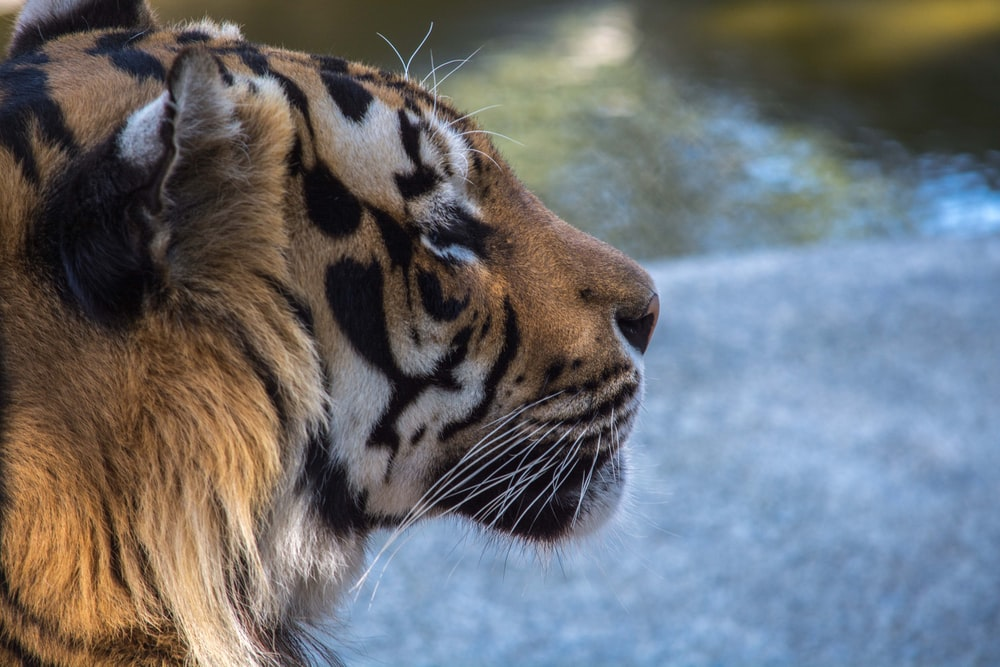
\includegraphics[width=.95\linewidth]{odiff1.jpg}\label{img:odiff1.jpg}
    \end{subfigure}%
    \begin{subfigure}{.33\textwidth}
        \centering
        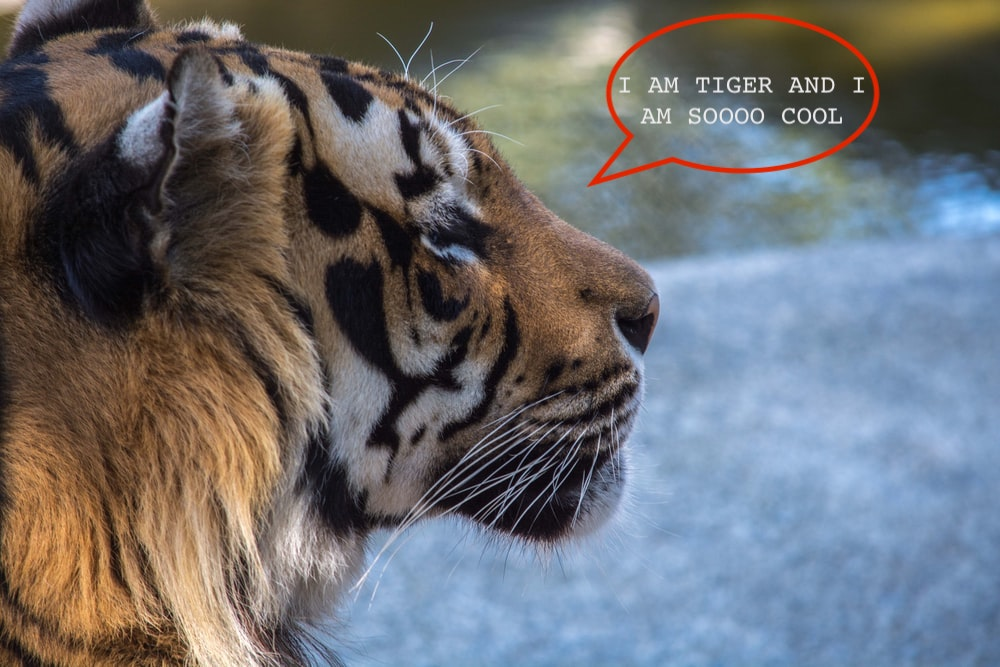
\includegraphics[width=.95\linewidth]{odiff2.jpg}\label{img:odiff2.jpg}
    \end{subfigure}%
    \begin{subfigure}{.33\textwidth}
        \centering
        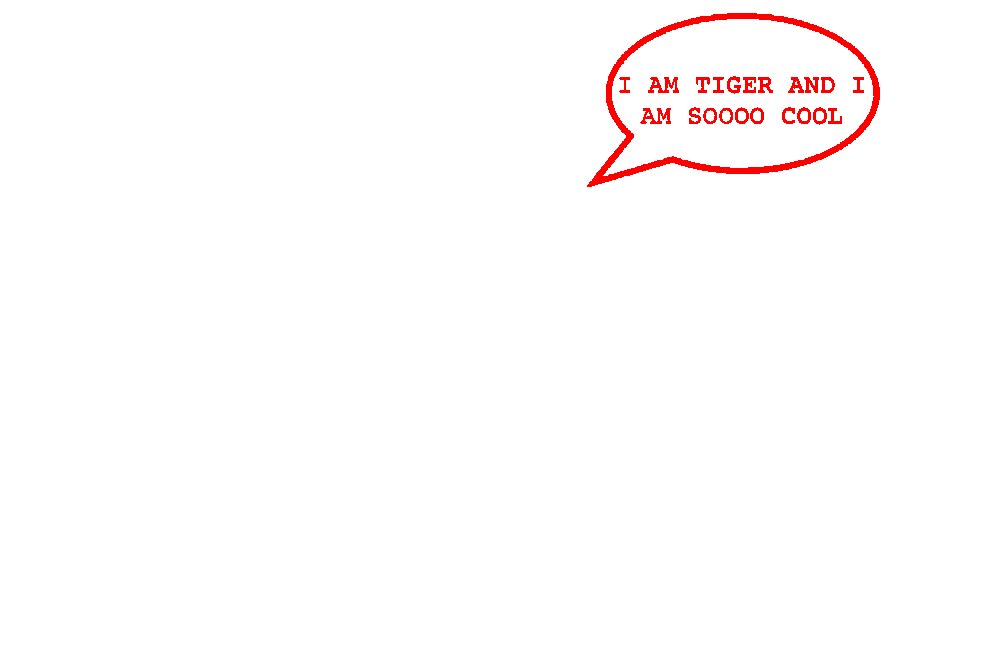
\includegraphics[width=.95\linewidth]{odiff3.png}\label{img:odiff3.png}
    \end{subfigure}
    \caption{Пример работы \textit{odiff}: эталон, паттерн, разница}\label{odiff}
}

\subsection{ImageDeDup}
\textit{ImageDeDup} -- это библиотека на языке \textit{Python}, предназначенная
для поиска и удаления дублирующихся изображений. Она расчитана исключительно на
работу с изображениями и может быть встроена в другие программы или
использоваться непосредственно в роли утилиты в \textit{REPL}"=оболочке
\cite{about-imagededup}.

Библиотека предлагает несколько методов сравнения:

\begin{itemize}
    \item Сверточные нейронные сети (\textit{CNN}) -- использование готовых моделей
          или собственных.
    \item Перцептивное хеширование (\textit{PHash})
    \item Хеширование разностей (\textit{DHash})
    \item Вейвлет"=хеширование (\textit{WHash})
    \item Хеширование по средним значениям разностей (\textit{AHash})
\end{itemize}

\textit{ImageDeDup}, в первую очередь, ориентирована на исследовательские нужды
и работу с нейронными сетями, например, с использованием библиотек
\textit{NumPy} и \textit{Jupyter}. По"=этому она предоставляет возможность
генерации совмещенных изображений для иллюстрации результатов сравнения.

Для практического использования библиотека требует определенных навыков
программирования на \textit{Python}, так как код для выбора исходных файлов и
определения удаляемых дубликатов необходимо писать самостоятельно. На рисунке
\ref{img:imagededup.png} показан пример применения библиотеки для составления
сравнительного изображения для некоторого изображения со всеми в указанном
каталоге.

\makeimage[Пример применения \textit{ImageDeDup}]{imagededup.png}

\subsection{Czkawka}
Изображенная на рисунке \ref{img:czkawka.png}, \textit{Czkawka} -- наследница
заброшенного с 2017 года проекта \textit{FSlint}. В отличии от оригинала на
\textit{Python2/GTK+2} и работающего только под линукс-системами, разработан на
\textit{Rust/GTK4} (альтернативный фронтенд написан на \textit{slint}) и
кроссплатформенна. Программа обеспечивает широкий спектр интрументов для
поддержания порядка в файловой системе: помимо дедубликации посредством
универсального хеширования, имеются отдельные обработчики фото, аудио и видео,
поиск пустых и временных файлов и каталогов, невалидных ссылок и имен, больших
файлов. Для сравнение изображений используется настраиваемый перцептивный хеш
\cite{about-czkawka}.

Параметры перцептивного хеша:

\begin{itemize}
    \item Алгоритм масштабирования изображения: Lanczos3, ближайший сосед,
          треугольный, гауссовский, алгоритм Катмалла"=Рома;
    \item Размер хеша: 8, 16, 32, 64;
    \item Тип хеша: одинарный, вертикальный, двойной градиентный, блочный,
          средний.
\end{itemize}

\makeimage[Интерфейс \textit{Czkawka}]{czkawka.png}

\section{Информационная база задачи}

\subsection{Сводка}
Единственная информация, которую сервис сравнения изображений может хранить
между сеансами -- его конфигурация и, если еспользуется хеширование, кеш,
включающий в себя путь к файлу, его хеш и дату последнего изменения или иные
метаданные, сигнализирующие об изменении файла для пересчета его хеш"=суммы.
Форматы файлов выбираются в зависимости от фреймворка и вкусов разработчика. В
данной работе -- \textit{csv}.

\subsection{Местоположение}
Местоположение файлов конфигурации в \textit{linux}: \textit{/etc} для
общесистемных файлов и каталог, хранимый в переменной
\textit{\$XDG\_CONFIG\_HOME} или \textit{\$HOME/.config}, если таковой не
определено, для пользовательских параметров \cite{xdg_base_directory_spec}.

Кеш, если его сохраненность между перезапусками системы не требуется,
традиционно хранится в каталоге \textit{/etc}, иначе в
\textit{\$XDG\_CACHE\_HOME} или \textit{\$HOME/.local/}, если такового не
определено \cite{xdg_base_directory_spec}.

\section{Функциональное назначение}

\subsection{Задача}
Главное назначение программы -- составление списков изображений на основании их
показателя сходства и его интерпретации с последующим экспортом или обработкой.

\subsection{Загрузка изображений}
Программа должна поддерживать самые популярные форматы изображений:
\textit{JPEG}, \textit{PNG}, \textit{TIFF}, \textit{BMP} и другие.

\subsection{Просмотр списка}
Важной функцией является просмотр списка сравниваемых изображений. В нем должна
отображаться информация об изображении, такая как название, показатели схожести,
размер файла, формат, дата съемки или любые иные полезные для пользователя
метаданные.

\subsection{Фильтрация}
Важной функцией является поиска по изображениям и сортировка их списка по
метаданным, таким как название, описание, теги, дата съемки, дата сохранения,
местоположение.

\subsection{Сравнение изображений}
Ключевой функцией программ для сравнения изображений является возможность
открывать и отображать два или более изображения одновременно для визуального
сравнения.

\subsection{Экспортирование списка}
Для пользователя будет очень удобна возможность экспорта списка сравниваемых
файлов с указанием экспортируемых полей списка, формата и пути, по которому он
будет сохранен. Форматами могут служить: \textit{JSON}, \textit{YAML},
\textit{CSV} и другие. Также можно реализовать генерацию скриптов для выполнение
каких"=либо действий над списком. К примеру, удаление дубликатов с показателем
схожести выше 98 процентов.

\subsection{Поддерживаемые платформы}
Поддержка \textit{linux} как целевой платформы.

\vspace{\baselineskip}
\phantomheading[section]{Заключение}

В разделе была рассмотрена задача о сравнение изображений, причины потребности
их сравнивать, существующие методы и программные решения. Помимо этого,
проведено их сравнение и оценена потребность в межсессионном хранении
информации, был составлен перечень требуемого функционала.
